\section{Design and Implementation}

\subsection{Overall power management design}

The aims set out for the preliminary design were to incorporate new batteries into Tiberius III, use more efficient motors, reduce the weight and improve the monitoring and control of the power from the various devices and motors that Tiberius would use.  These features were implemented with varying degrees of success.  
The weight was dramatically reduced due to the restructuring of the chassis by removing about half of the aluminium extrusion, the various mountings and battery holders were all 3D printed using lightweight PLA, the batteries themselves were also significantly lighter than the previous versions.  However, the total weight reduction ended up being quite small due to the additional hardware including a robotic arm which added quite a bit of weight.  

The control Raspberry Pi had a power management module that allowed it to monitor and control the different components and even turn parts of the vehicle off, including the Kinect 2 sensor and processor, the robotic arm and even the ability to shut down the motors if necessary.  
Relays were used to allow the Kinect 2, the motors and the robotic arm which are controlled by the control pi and can turn off those components in low power mode.  

\begin{figure}[!htb]
\begin{center}
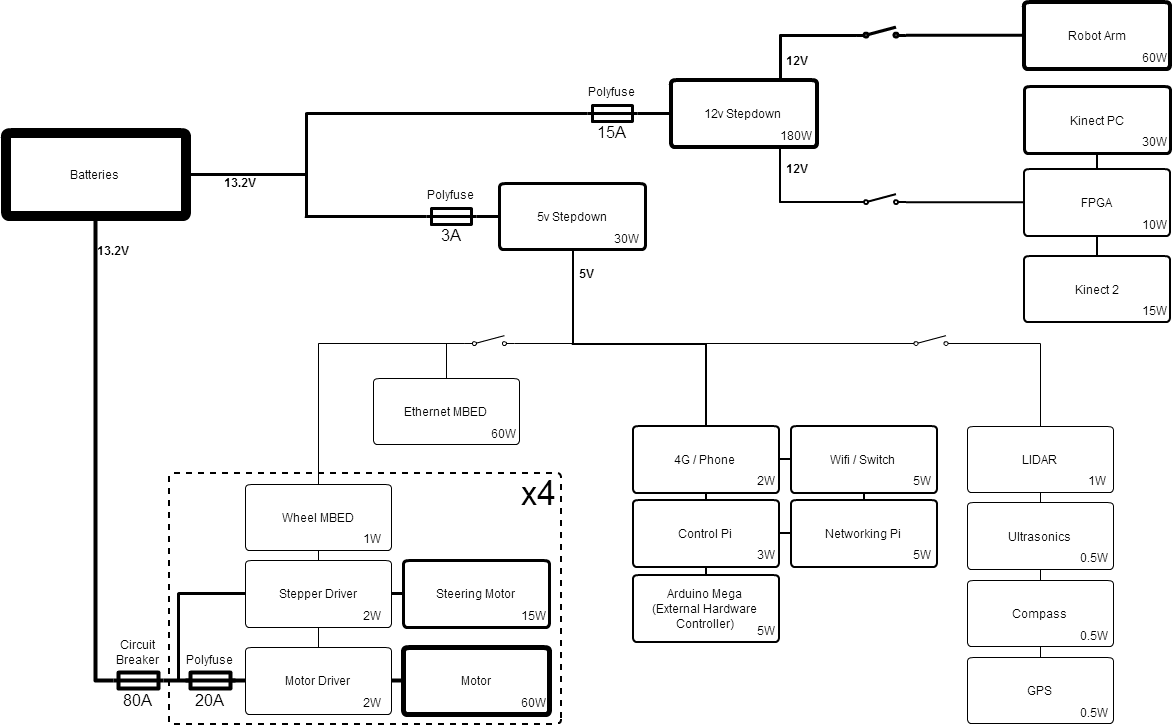
\includegraphics[width=15cm]{power.png}
\end{center}
\caption{Initial Power Management Design}
\label{fig:power}
\end{figure}

\subsection{Power monitoring and usage}
Two specialised current sensing boards were used to measure the current being used from the batteries as well as the voltage. The boards were connected to an mbed which calculated the current power consumption, and total used power in amp-hours and watt-hours.

This monitoring can then be used to work out if Tiberius can complete a mission without running out of power.
